\documentclass[a4paper]{article}

\usepackage[top=3.5cm, bottom=3.5cm, left=3.5cm, right=3.5cm]{geometry}
\usepackage{ae,lmodern}
\usepackage[english]{babel}
\usepackage[utf8]{inputenc}
\usepackage[T1]{fontenc}

%\usepackage{paralist, tabularx}
\usepackage{oldlfont,amssymb,epsf,stmaryrd,epsfig,color}\usepackage{amsmath}
%\usepackage{hyperref}
%\usepackage{framed,multicol,changepage}
%\usepackage{graphicx}
\usepackage[dvipsnames]{xcolor}
%\usepackage{skull,ifoddpage,marginnote}
%\usepackage{pifont}
%\usepackage{graphicx}
%\usepackage{ebproof}
%\usepackage{mathtools}
%\usepackage{bm}
%\usepackage{stmaryrd}
%\usepackage{cleveref}
\usepackage{tikz}
%\usepackage{import} % For inkscape generated files
\usepackage{biblatex}
\usepackage{url}

\title{Title}
\date{}

\def\Type{\mbox{\tt TYPE}}
\def\Kind{\mbox{\tt KIND}}
\def\ra{\rightarrow}
\def\lra{\longrightarrow}
\def\Set{\mbox{\it Set}}
\def\bliota{{\color{blue} ind}}
\def\El{{\mbox{\it El}}}
\def\Prop{{\mbox{\it Prop}}}
\def\Prf{{\color{blue} \mbox{\it Prf}}}
\def\imp{\mathbin{\color{blue} \Rightarrow}}
\def\fa{{\color{blue} \forall}}
\def\bltop{{\color{blue} \top}}
\def\blbot{{\color{blue} \bot}}
\DeclareMathOperator{\blneg}{{\color{blue} \neg}}
\def\conj{\mathbin{\color{blue} \wedge}}
\def\disj{\mathbin{\color{blue} \vee}}
\def\ex{{\color{blue} \exists}}
\def\S{{\color{blue} \mbox{\it succ}}}
\def\0{{\color{blue} 0}}
\def\positive{{\color{blue} \mbox{\it positive}}}
\def\pred{{\color{blue} \mbox{\it pred}}}
\def\Prfc{{\color{blue} \mbox{\it Prf}_c}}
\def\impc{\mathbin{\color{blue} \Rightarrow_c}}
\def\conjc{\mathbin{\color{blue} \wedge_c}}
\def\disjc{\mathbin{\color{blue} \vee_c}}
\def\fac{{\color{blue} \forall_c}}
\def\exc{{\color{blue} \exists_c}}
\def\o{{\color{blue} o}}
\def\arr{\mathbin{\color{blue} \leadsto}}%\mbox{\it arrow}}}
\def\arrd{\mathbin{\color{blue} \leadsto_d}}%\mbox{\it arrow}_d}}
\def\impd{\mathbin{\color{blue} \Rightarrow_d}}
\def\blpi{{\color{blue} \pi}}
\def\Scheme{{\color{blue} \mbox{\it Scheme}}}
\def\Els{{\color{blue} \mbox{\it Els}}}
\def\lift{{\color{blue} \uparrow}}
\def\calfa{{\rotatebox[origin=c]{180}{{\color{blue} A}}}}
\def\sffa{{\rotatebox[origin=c]{180}{{\color{blue}\ensuremath{\mathcal{A}}}}}}
\def\pos{\mbox{\it positive}}
\def\psub{{\color{blue} \mbox{\it psub}}}
\def\pair{{\color{blue} \mbox{\it pair}}}
\def\fst{{\color{blue} \mbox{\it fst}}}
\def\snd{{\color{blue} \mbox{\it snd}}}
\def\eq{{\mbox{\it eq}}}
\def\refl{{\mbox{\it refl}}}

\newtheorem{definition}{Definition}[section]
\newtheorem{theorem}{Theorem}[section]
\newtheorem{lemma}{Lemma}[section]
\newtheorem{corollary}{Corollary}[section]
\newtheorem{property}{Property}[section]

\newenvironment{proof}{\noindent {\em Proof.}}{\medskip}
\newenvironment{example}{\noindent {\em Example.}}{\medskip}
\newenvironment{remark}{\noindent {\em Remark.}}{\medskip}

\colorlet{ftcolor}{Aquamarine}

\newcommand{\mute}[1]{\ifdraft{#1} \else{} \fi}

\newcounter{WarnCounts}
\newcommand{\decorateWC}{
  \stepcounter{WarnCounts}
  \checkoddpage
  \ifoddpageoroneside
     \mbox{}\marginnote{\textcolor{red}{$\skull_{\theWarnCounts}$}}
     \else
     \reversemarginpar
     \mbox{}\marginnote{\textcolor{red}{$\skull_{\theWarnCounts}$}}
     \normalmarginpar
   \fi
}

\newcounter{ToDos}
\newcommand{\decorateTD}{
  \stepcounter{ToDos}
    \checkoddpage
    \ifoddpageoroneside
     \mbox{}\marginnote{\textcolor{red}{$\skull_{\theToDos}$}}
     \else
     \reversemarginpar
     \mbox{}\marginnote{\textcolor{red}{$\skull_{\theToDos}$}}
     \normalmarginpar
   \fi
}

% Skeleton for remark comments
% 1: Name, 2: Color, 3:Comment
\newcommand{\signedComment}[3]
           {\mute{\decorateWC\textcolor{#2}{(#1:~{#3})}}}

% remarks
\newcommand{\todo}[1]{\mute{\decorateTD\textcolor{red}{(TODO:~{#1})}}}

\colorlet{ftcolor}{Aquamarine}
\colorlet{fbcolor}{LimeGreen}
\colorlet{gdcolor}{RawSienna}
\colorlet{egcolor}{Plum}
\colorlet{ghcolor}{Orange}

\newcommand{\ft}[1]{\signedComment{FT}{ftcolor}{#1}}
\newcommand{\fb}[1]{\signedComment{FB}{fbcolor}{#1}}
\newcommand{\gd}[1]{\signedComment{GD}{gdcolor}{#1}}
\newcommand{\eg}[1]{\signedComment{EG}{egcolor}{#1}}
\newcommand{\gh}[1]{\signedComment{GH}{ghcolor}{#1}}

\newcommand{\cF}{\mathcal{F}}


\newcommand{\CF}{\mathcal{F}}
\newcommand{\CP}{\mathcal{P}}
\newcommand{\CT}{\mathcal{T}}

\newcommand{\systemstyle}[1]{\textsc{#1}}

\newcommand{\coc}{\systemstyle{Calculus of Constructions}}
\newcommand{\dedukti}{\systemstyle{Dedukti}}
\newcommand{\lc}{\systemstyle{\ensuremath{\lambda\text{-calculus}}}}
\newcommand{\lcs}{\systemstyle{\ensuremath{\lambda\text{-calculi}}}}
\newcommand{\lpc}{\systemstyle{\ensuremath{\lambda \Pi\text{-calculus}}}}
\newcommand{\lpcm}{\systemstyle{\ensuremath{\lambda \Pi\text{-calculus modulo theory}}}}
\newcommand{\lprolog}{\systemstyle{\ensuremath{\lambda\text{-Prolog}}}}



\def\Graph{{\mbox{\it Graph}}}
\def\Node{{\mbox{\it Node}}}
\def\omicron{{\mbox{\it omicron}}}
\def\arr{{\mbox{\it arrow}}}
\input{lambdapi.tex}
\addbibresource{ref.bib}

\begin{document}
\thispagestyle{empty}
\maketitle

\section{Introduction}

\dedukti \ is a logical framework based upon the language \lpcm, which was created to overcome the lack of interoperability between proof assistanrs. As it is a logical framework, we can implement in \dedukti \ theories. Especially, \textit{Set theory} is interesting beacause it will enable traductions from and towards \textsc{Isabelle/ZF}.

A previous work \cite{zermodulo} has demonstrate the implemtation of \textit{Set theory} in \textit{Deduction modulo} thaks to a structure of \textit{pointed graphs}. Until the writing of \cite{zermodulo}, \lpcm \ has been created as an improvement of \textit{Deduction modulo}. We adapt the implementation to the \lpcm \ and then implement it in \dedukti. 

\section{The theory of pointed graphs}

To implement $Set \ theory$ in \dedukti, the first idea is to translate the axioms of the theory into rewriting rules. Nevertheless, as pointed out by M. Crabbé \cite{crabbé}, such implementation does not guarantee normalization. That is why A. Miquel and G. Dowek \cite{zermodulo} introduced a theory of pointed graphs such that the implementation of $Set~theory$ respects normalization.

\subsection{Pointed graphs}

Sets are reprented by pointed graphs. A pointed graph is characterizd by a direct graph and one of its node identified as the root. 

\begin{figure}[h]
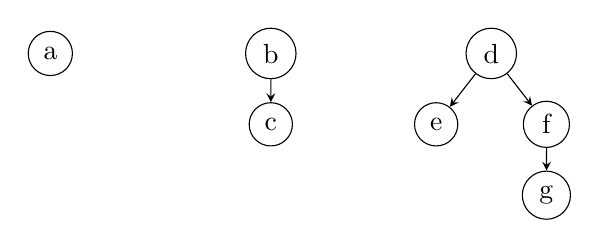
\begin{tikzpicture}[>=stealth,yscale=1.8,xscale=1.4]  

\node(a) at (3,3)[circle,draw,text centered] {a};
\node(b) at (5,3)[circle,draw,text centered] {b};
\node(c) at (5,2.5)[circle,draw,text centered] {c};
\node(d) at (7,3)[circle,draw,text centered] {d};
\node(e) at (6.5,2.5)[circle,draw,text centered] {e};
\node(f) at (7.5,2.5)[circle,draw,text centered] {f};
\node(g) at (7.5,2)[circle,draw,text centered] {g};
                      
\draw[->] (b) -- (c); 
\draw[->] (d) -- (e);
\draw[->] (d) -- (f);
\draw[->] (f) -- (g);

\end{tikzpicture}
\end{figure}

The first graph with root $a$ represents the set $\emptyset$. The second graph with root $b$ represents the set $\{\emptyset\}$, while with root c it represents $\emptyset$. The third graph with root $d$ represents $\{\emptyset,\{\emptyset\}\}$, \textit{etc}.

The operator $root$ gives the root of a pointed graph. $a/x$ replace the root of $a$ by $x$. $x \eta_a y$ means there is a edge in $a$ from $y$ to $x$. $rel(x,y,r)$ means that $x$ and $y$ are related by the relation $r$.

Because some different pointed graphs represents the same set, we introduce the bisimilarity: 

$a \simeq b \lra \ex r~(rel(root(a),root(b),r) \\
\conj \ \fa x \fa x'~\fa y~(x'~\eta_a~x~\conj~rel(x, y, r)~\imp~\ex~y'~(y'~\eta_b~y~\conj~rel(x', y', r))) \\
\conj \ \fa y \fa y'~\fa x~(y'~\eta_b~y~\conj~rel(x, y, r)~\imp~\ex~x'~(x'~\eta_a~x~\conj~rel(x', y', r))))$

\subsection{The theory IZmod}

IZmod


\section{The language of pointed graphs}

\subsection{Sorts}

The langage of the theory IZmod uses four sorts. The first two are for
the pointed graphs and for the nodes of the pointed graphs.  In
\dedukti, we would need two universal quantifiers and two
existential quantifiers, one for each sort.  We rather use another
solution \cite{theoryU} that is to declare a constant $\Set$ of type
$\Type$ for codes of sorts, a function $\El$ of type $\Set \ra \Type$,
two constants $graph$ and $node$ of sort $\Set$.

\begin{lstlisting}
constant symbol graph : Set;
constant symbol node : Set;
\end{lstlisting}

The two other sorts of the theory IZmod are for classes of nodes and
for binary relations on nodes.  In \dedukti, the sort of classes is
just $\El~node \ra \El~prop$ and that of binary relations
$\El~node \ra \El~node \ra \El~prop$. To quantify on such sorts, we introduce constant $\arr $ of type
$\Set \ra \Set \ra \Set$ and rewrite rule
$$\El~(x~\arr~y) \lra (\El~x) \ra (\El~y)$$

The symbols $graph$ and $node$ are specific to the
expression of $IZmod$ in \dedukti. In contrast the symbols $\Set$,
$\El$, $prop$, and $\arr$ are part of the standard library of 
\dedukti.

\subsection{Signature}

The signature of $IZmod$ contains 31 symbols. As we have replaced the
sorts for classes and relations with the \dedukti \ types
$\El~node \ra \El~prop$ and $\El~node \ra \El~node \ra \El~prop$, we do not need specific predicate symbols to apply a class to a node or a relations to two. In the same way, we do not need comprehension axioms for classes and relations. 

Similarly, the equality symbol is part of the standard library of \dedukti.

So the signature is reduced to 26 symbols. The specific case of the comprehension symbol is treated later.

\begin{lstlisting}
symbol eta : El graph → El node → El node → El prop;
symbol root : El graph → El node;
symbol cr : El graph → El node → El graph;
constant symbol o : El node;
constant symbol O : El node;
symbol i : El node → El node;
symbol i' : El node → El node;
symbol j : El node → El node;
symbol j' : El node → El node;
symbol I : El node → El prop;
symbol J : El node → El prop;
symbol ρ : El graph → El node;
symbol ρ^ : El node → El graph;
symbol Succ : El node → El node;
symbol Pred : El node → El node;
symbol Null : El node → El prop;
symbol Nat : El node → El prop;
symbol < : El node → El node → El prop;
symbol simeq : El graph → El graph → El prop;
symbol ∈ : El graph → El graph → El prop;
symbol join : El graph → El graph;
symbol pair : El graph → El graph → El graph;
symbol powerset : El graph → El graph;
symbol omega : El graph;
symbol Cl : El graph → El graph;
\end{lstlisting}

\subsection{From \textit{Deduction modulo} to \lpcm}

Since the publication of \cite{zermodulo}, \lpcm has been developped as an evolution of \textit{Deduction modulo}.

More specifically, \lpcm allows to quantify on proposition.

In \dedukti, the symbol $mem$ and $rel$ are useless. Indeed, we can apply a node $x$ to class $P$ with $P~x$ and two nodes $x$ and $y$ to a relation $r$ with $r~x~y$.


\subsection{Rewriting rules}

The rewriting rule $$y = z \ \lra \ \fa \ p \ (mem(y, p) \ \imp \ mem(z, p))$$ is not required as it is a consequence of the rewriting rule of the polymorphic $=$ implemented in the stardard library of \dedukti: 
\begin{lstlisting}
constant symbol = [s] : El s → El s → El prop;
notation = infix 4;
rule π (@= $s $x $y) ↪ Π (P : El $s → El prop), π(P $x) → π(P $y);
\end{lstlisting}

+ Expliquer pourquoi on n'utilise pas les symboles g et g' \\

All the other rewriting rules, except the ones involving $comp$, are easy to implement in \dedukti.

\begin{lstlisting}
rule eta (cr $a $z) $x $y ↪ eta $a $x $y;
rule root (cr $a $x) ↪ $x;
rule (cr (cr $a $x) $y) ↪ cr $a $y;

rule i' (i $x) ↪ $x;
rule j' (j $x) ↪ $x;
rule ρ^ (ρ $x) ↪ $x;
rule I (i $x) ↪ ⊤;
rule J (j $x) ↪ ⊤;
rule I (j $x) ↪ ⊥;
rule J (i $x) ↪ ⊥;
rule I (o) ↪ ⊥;
rule J (o) ↪ ⊥;

rule Pred (Succ $x) ↪ $x ;
rule Null O ↪ ⊤;
rule Nat O ↪ ⊤;
rule Null (Succ $x) ↪ ⊥;
rule Nat (Succ $x) ↪ Nat $x;

rule $x < O ↪ ⊥;
rule $x < (Succ $y) ↪ ($x < $y) ∨ ($x = $y);

rule $a simeq $b ↪ `∃ r : El (node arrow (node arrow prop)), 
    r (root $a) (root $b)
    ∧ (`∀ x, `∀ x', `∀ y, 
        eta $a x' x ∧ r x y
            ⇒ `∃ y', eta $b y' y ∧ r x' y')
    ∧ (`∀ y, `∀ y', `∀ x, 
        eta $b y' y ∧ r x y
            ⇒ `∃ x', eta $a x' x ∧ r x' y');

rule $a ∈ $b ↪ `∃ x, ((eta $b x (root $b)) ∧ ($a simeq cr $b x));

rule eta (join $a) $x $x' ↪ 
	(`∃ y, `∃ y', ($x = i y) ∧ ($x' = i y') ∧ eta $a y y')
    ∨ (`∃ y, `∃ z, ($x = i y) 
    	∧ ($x' = o) 
    	∧ eta $a y z 
    	∧ eta $a z (root $a));

rule eta (pair $a $b) $x $x' ↪ 
	(`∃ y, `∃ y', (($x = i y) ∧ ($x' = i y') ∧ eta $a y y'))
    ∨ (`∃ y, `∃ y', ($x = j y) ∧ ($x' = j y') ∧ eta $b y y')
    ∨ (($x = i (root $a)) ∧ ($x' = o))
    ∨ (($x = j (root $b)) ∧ ($x' = o));

rule eta (powerset $a) $x $x' ↪ 
	(`∃ y, `∃ y', ($x = i y) ∧ ($x' = i y') ∧ eta $a y y')
    ∨ (`∃ y, `∃ c, ($x = i y) 
    	∧ ($x' = j (ρ c)) 
    	∧ (eta $a y (root $a)) 
    	∧ ((cr $a y) ∈ c))
    ∨ (`∃ c, ($x = j (ρ c)) ∧ ($x' = o));

symbol omega : El graph;
rule eta omega $x $x' ↪ 
	(`∃ y, `∃ y', ($x = i y) ∧ ($x' = i y') ∧ (y < y'))
    ∨ (`∃ y, ($x = i y) ∧ ($x' = o) ∧ Nat y);

rule eta (Cl $a) $x $x' ↪ 
	(`∃ y, `∃ y', (($x = i y) ∧ ($x' = i y') ∧ eta $a y y'))
    ∨ (`∃ y, ($x = i y) 
        ∧ ($x' = o)
        ∧ (`∀ c : El (node arrow prop), 
                ((`∀ z, eta $a z (root $a) ⇒ c z)
                ∧ (`∀ z, `∀ z', (eta $a z z') ∧ (c z') ⇒ (c z)))
            ⇒ c y));
            
rule root (join $a) ↪ o;
rule root (pair $a $b) ↪ o;
rule root (powerset $a) ↪ o;
rule root omega ↪ o;
rule root (Cl $a) ↪ o;

\end{lstlisting}


\section{The language of formulas}

We may have notice that the lemmas in which the $comp$ symbol is used are only valid for a subset of formulas. The formulas need to have all of its quantifiers of sort $El~graph$ and can only use the language $\in$, $\simeq$ and the classic logical connectives.

Thus we need to introduce a set to caraterize the validity domain of such lemmas.

\subsection{Formulas}

In order to achieve this goal, we define the constant $formula$ of type $\Set$ and the logical connectives related to this constant.

\begin{lstlisting}
constant symbol formula : Set;
constant symbol eqF : El nat → El nat → El formula;
constant symbol inF : El nat → El nat → El formula;
constant symbol andF : El formula → El formula → El formula;
constant symbol orF : El formula → El formula → El formula;
constant symbol allF : El nat → El formula → El formula;
constant symbol exF : El nat → El formula → El formula;
constant symbol impF : El formula → El formula → El formula;
constant symbol fF : El formula;
constant symbol tF : El formula;
\end{lstlisting}

Then we are able to define an induction over formulas, using the language $\in$, $\simeq$ and the classic logical connectives.

\begin{lstlisting}
constant symbol recF : Π (P : El formula → Prop), 
π(`∀ x, `∀ y, P (eqF x y))
→ π(`∀ x, `∀  y, P (inF x y))
→ π(`∀ f, `∀ g, (P f ∧ P g) ⇒ (P (andF f g)))
→ π(`∀ f, `∀ g, (P f ∧ P g) ⇒ (P (orF f g)))
→ π(`∀ f, `∀ g, (P f ∧ P g) ⇒ (P (impF f g)))
→ π(`∀ f, (P f) ⇒ (`∀ x, P (allF x f)))
→ π(`∀ f, (P f) ⇒ (`∀ x, P (exF x f)))
→ π(P tF)
→ π(P fF)
→ π(`∀ f, P f);
\end{lstlisting}

\subsection{Interpretation}

The next step is to interpret an object of type $formula$ into $Prop$. We introduce the constant $interpretation$ which receives a valuation of type $\El \ nat \ \ra \ \El~graph$ and a formula of type $\El \ formula$ and return a $\El~prop$.

\begin{lstlisting}
symbol interpretation : (El nat → El graph) → El formula → El prop;
\end{lstlisting} 

We need to have a tool to update a valuation when we assign a variable. To do so, we introduce the constant $update$ of type $(\El \ nat \ra \El~graph) \ra \El \ nat \ra \El~graph \ra (\El \ nat \ra \El~graph)$ which takes as arguments a valuation $\sigma$, a natural number $x$ and a graph $a$ and returns a new valuation $(update \ \sigma \ x \ a)$ that substitues $x$ by $a$ and acts like $\sigma$ for the other natural numbers.

To write a rewriting rule upon $update$, we need to be able to check if we apply $(update \ \sigma \ x \ a)$ to $z = x$ or to $z \neq x$.

We define the symbol $update1$ of type $(\El \ nat \ \ra \ \El~graph) \ \ra \ \El \ nat \ \ra \ \El~graph \ \ra \ \El \ nat \ \ra \ (\El \ nat \ \ra \ \El~graph)$. The new argument $z$ is used to keep in memory the argument $y$:

$$update \ \sigma \ x \ a \ y \ \lra \ update1 \ \sigma \ x \ a \ y \ y$$

We have two natural numbers to compare: $x$, which is substitued by $a$, and $y$ that is the argument we apply to the valuation. The technique we use to compare $x$ and $y$ is the following: 

\begin{itemize}
\item We keep in memory $y$ in the variable $z$;
\item We decrement $x$ and $y$ until either one or both are equal to zero;
\item If both are equal to zero, then $x$ and $y$ are equal and we return $a$. If only one equals zero, then they are different and we return $\sigma \ z$.
\end{itemize}

$$update1 \ \sigma \ (s \ x) \ a \ (s \ y) \ z \ \lra \ update1 \ \sigma \ x \ a \ y \ z$$
$$ update1 \ \sigma \ zero \ a \ zero \ z \ \lra \ a$$
$$update1 \ \sigma \ zero \ a \ (s \ y) \ z \ \lra \ \sigma \ z$$
$$update1 \ \sigma \ (s \ x) \ a \ zero \ z \ \lra \ \sigma \ z$$


Now we have all the tools to define the rewiting rules of the interpreation of formulas:

$$interpretation \ \sigma \ (eqF \ x \ y) \lra (\sigma \ x) \ \simeq \ (\sigma \ y)$$
$$interpretation \ \sigma \ (inF \ x \ y) \lra (\sigma \ x) \ \in \ (\sigma \ y)$$
$$interpretation \ \sigma \ (andF \ f \ g) \lra (interpretation \ \sigma \ f) \conj (interpretation \ \sigma \ g)$$
$$interpretation \ \sigma \ (orF \ f \ g) \lra (interpretation \ \sigma \ f) \disj  (interpretation \sigma \ g)$$
$$interpretation \ \sigma \ (impF \ f \ g) \lra (interpretation \ \sigma \ f) \imp (interpretation \ \sigma \ g)$$
$$interpretation \ \sigma \ (allF \ x \ f) \ \lra \ \fa \ a, interpretation \ (update \ \sigma \ x \ a) \ f$$
$$interpretation \ \sigma \ (exF \ x \ f) \ \lra \ \ex \ a, interpretation \ (update \ \sigma \ x \ a) \ f$$
$$interpretation \ \sigma \ fF \lra \blbot$$
$$interpretation \ \sigma \ tF \lra \bltop$$

\subsection{Comprehension and infinity}

Henceforth, we are able to define in \dedukti
$$comp : \El~graph \ra (\El \ nat \ \ra \ \El~graph) \  \ra \El \ formula \ra \ \El~graph$$

and its rewriting rules

\begin{lstlisting}
rule eta (comp $a $σ $f) $x $x' ↪ 
(`∃ y, `∃ y', (($x = i y) ∧ ($x' = i y') ∧ eta $a y y')) 
∨ (`∃ y, ($x = i y) ∧ ($x' = o) ∧ (eta $a y (root $a))
∧ (interpretation (update $σ zero (cr $a y)) $f));
rule root (comp $a $σ $f) ↪ o;
\end{lstlisting}

When it comes to symbol related to the Infinity section of \cite{zermodulo}, we implement $empty_set$ of type $\El~graph$ and $Ind$ of type $\El~graph \ \ra \ \El~prop$.

To define the empty set, we use $comp$ with the formula $fF$:
\begin{lstlisting}
rule empty_set ↪ comp omega (λ _, empty_set) fF;
rule root empty_set ↪ o;
\end{lstlisting}

Then we implement

\begin{lstlisting}
rule Ind $c ↪ (empty_set ∈ $c) 
∧ (`∀ a, (a ∈ $c) ⇒ ((join (pair a (pair a a))) ∈ $c));
\end{lstlisting}


\subsection{Results concerning valuation}

Thanks to the introduction of $interpretation$, we can deduce five theorems. \\

The first theorem is used to simplify the terms when updating a valuation.

\begin{theorem}
$\fa \ \sigma, \fa \ x, y, z, \fa \ a, [(eqNP \ x \ y) \ \imp \ (((update1 \ \sigma \ x \ a) \ y \ z) \ \simeq \ a)] \ \conj \ [\blneg(eqNP \ x \ y) \ \imp \ (((update1 \ \sigma \ x \ a) \ y \ z) \ \simeq \ (\sigma \ z))]$
\end{theorem}

\begin{proof}
The first term of the conjonction is proved by simple recurrence over natural numbers. The second term of the conjonction is proved by double recurrence.
\end{proof}

The second theorem conveys the idea that if two graphs are bisimilar then it is identical to update a valuation by either of theses two graphs.

\begin{theorem}
$\fa \ \sigma, \fa \ x, \fa \ a, b, (a \ \simeq \ b) \ \imp \ [\fa y, (update \ \sigma \ x \ a \ y) \ \simeq \ (update \ \sigma \ x \ b \ y)]$
\end{theorem}

\begin{theorem}
$\fa \ \sigma, \fa \ x, y, \fa \ a, b, c, (a \ \simeq \ b) \ \imp \ (\fa z, (update \ (update \ \sigma \ x \ a) \ y \ c \ z) \ \simeq \ (update \  (update \ \sigma \ x \ b) \ y \ c \ z))$
\end{theorem}

The fourth theorem states that if two valuations are equal they keep being equal after an update.

\begin{theorem}
$\fa \ \sigma, \sigma', \fa \ x, \fa \ c, (\fa y, \sigma \ y \ \simeq \ \sigma' \ y) \ \imp \ (\fa z, (update \ \sigma \ x \ c \ z) \ \simeq \ (update \ \sigma' \ x \ c \ z))$
\end{theorem}

\begin{theorem}
$\fa \ f, \fa \ \sigma, \sigma', (interpretation \ \sigma \ f) \ \conj \ (\fa x, (\sigma \ x) \ \simeq \ (\sigma' \ x))) \ \imp \ (interpretation \ \sigma' \ f)$
\end{theorem}

\begin{proof}
The fifth theorem is proved by induction over formulas.
\end{proof}

\section{Lemmas}

The first lemma $x=x$ does not need to be implemented since it is already part of the standard library of \dedukti \ under the name $refl$ (which is polymorphic).


\subsection{Useful mechanisms}

All the other lemmas except the ones where $comp$ is involved are proved using the blueprint in \cite{zermodulo53}. The complete proofs can be found in \url{https://github.com/ttraversie/zf/tree/main/theoriezf}.

\subsection{Some interesting proofs}

Lemma32 + utilisation du lemma32

\subsection{Weak extensionnality}

We notice in \cite{zermodulo53} the use of \textit{weak extensionality} to prove lemmas 44, 47 and 48. We want to deduce \textit{weak extensionality} from \textit{strong extensionality} (i.e. lemma 41).

To do this, we need to prove the following intermediary lemma:

\begin{lstlisting}
opaque symbol lemmaHypExt : Π (c d : Graph), π((`∀ z, (z ∈ c) ⇔ (z ∈ d)) ⇒ ((((c simeq c) ∧ (d simeq d)) ∨ (c simeq d))
∧ (`∀ a, `∀ a', `∀ b, ((a' ∈ a) ∧ (((a simeq c) ∧ (b simeq d)) ∨ (a simeq b))) ⇒ (`∃ b', ((b' ∈ b) ∧ (((a' simeq c) ∧ (b' simeq d)) ∨ (a' simeq b')))))
∧ (`∀ b, `∀ b', `∀ a, ((b' ∈ b) ∧ (((a simeq c) ∧ (b simeq d)) ∨ (a simeq b))) ⇒ (`∃ a', ((a' ∈ a) ∧ (((a' simeq c) ∧ (b' simeq d)) ∨ (a' simeq b')))))))
\end{lstlisting}

We thus can prove $weak \ extensionality$ thanks to:

\begin{lstlisting}
opaque symbol lemmaExt : Π (c d : Graph), π((`∀ x, (x ∈ c) ⇔ (x ∈ d)) ⇒ (c simeq d))
≔ begin
assume c d H;
refine lemma41 zero one (orF (andF (eqF zero two) (eqF one three)) (eqF zero one)) c d (update (update (λ _, empty_set) two c) three d) (lemmaHypExt c d H);
end;
\end{lstlisting}

\section{Conclusion}

Schema pour représenter Z, Zmod et ZF ?

\begin{center}
\begin{tabular}{|c|c||c|c|}
\hline Lemma & Number of lines in the proof & Lemma & Number of lines in the proof \\
\hline 3 & ? & 29 & ? \\
\hline 4 & ? & 30 & ? \\
\hline 5 & ? & 31 & ? \\
\hline 6 & ? & 32 & ? \\
\hline 7 & ? & 33 & ? \\
\hline 8 & ? & 34 & ? \\
\hline 9 & ? & 35 & ? \\
\hline 10 & ? & 36 & ? \\
\hline 11 & ? & 37 & ? \\
\hline 12 & ? & 38 & ? \\
\hline 13 & ? & 39 & ? \\
\hline 14 & ? & 40 & ? \\
\hline 15 & ? & 41 & ? \\
\hline 16 & ? & 42 & ? \\
\hline 17 & ? & 43 & ? \\
\hline 18 & ? & 44 & ? \\
\hline 19 & ? & 45 & ? \\
\hline 20 & ? & 46 & ? \\
\hline 21 & ? & 47 & ? \\
\hline 22 & ? & 48 & ? \\
\hline 23 & ? & 49 & ? \\
\hline 24 & ? & 50 & ? \\
\hline 25 & ? & 51 & ? \\
\hline 26 & ? & 52 & ? \\
\hline 27 & ? & 53 & ? \\
\hline 28 & ? & Weak extensionality & ? \\
\hline
\end{tabular}
\end{center}

\printbibliography

\end{document}